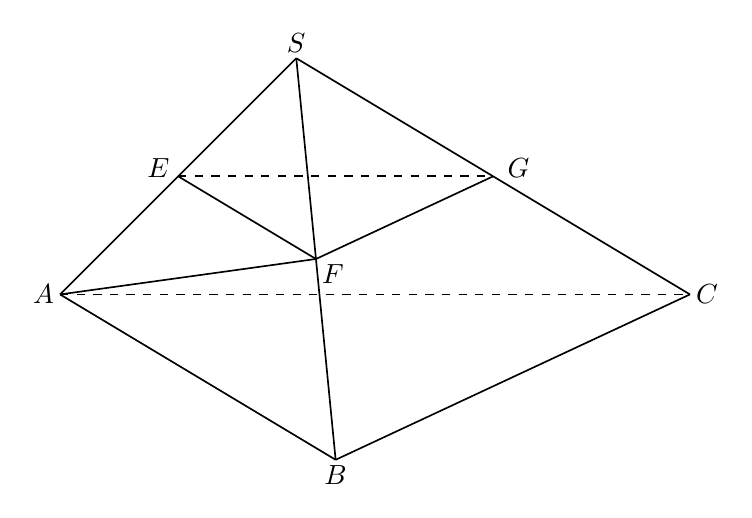
\begin{tikzpicture}[x=1cm,y=1cm,font=\normalsize,
  edge/.style={draw=black,solid,line width=.6pt},
  hide/.style={draw=black,dashed,line width=.6pt}]
% S-ABC tetrahedron: E,F,G midpoints of SA,SB,SC
\coordinate (S) at (3.0,4.5);
\coordinate (A) at (0.0,1.5);
\coordinate (B) at (3.5000000000,-0.6000000000);
\coordinate (C) at (8.0,1.5);
\coordinate (E) at (1.5,3.0);
\coordinate (F) at (3.2500000000,1.9500000000);
\coordinate (G) at (5.5,3.0);
% solid outline and interior
\draw[edge] (S)--(A);
\draw[edge] (S)--(F);
\draw[edge] (F)--(B);
\draw[edge] (S)--(G);
\draw[edge] (G)--(C);
\draw[edge] (A)--(B);
\draw[edge] (B)--(C);
\draw[edge] (E)--(F);
\draw[edge] (F)--(G);
\draw[edge] (A)--(F);
% hidden: base AC and midline EG
\draw[hide] (A)--(C);
\draw[hide] (E)--(G);
% labels offset from strokes
\node[above,inner sep=2pt] at (S) {$S$};
\node[left,inner sep=2pt,xshift=-1pt,yshift=3pt] at (E) {$E$};
\node[right,inner sep=2pt,xshift=3pt,yshift=3pt] at (G) {$G$};
\node[left,inner sep=2pt] at (A) {$A$};
\node[below,inner sep=2pt] at (B) {$B$};
\node[right,inner sep=2pt] at (C) {$C$};
\node[below right,inner sep=2pt] at (F) {$F$};
\end{tikzpicture}
